\chapter{Problem definition}
One edge of Medialogy is systems build to reach accordingly to humans this is called Visual Computing. There are several not least good topics that apply to this kind of technology/work areas. One area in which image processing and specific object recognition is used is surveillance. By implementing some custom made software, one will be able to monitor a specific target group or process. 

Simultaneously three groups each year on the third semester of Medialogy is selected to collaborate with Hjørring Library in creating some intuitive interface that will react to humans. It was decided within the group that it was of interest to work with Hjørring Library, therefore an application was sent to the semester coordinator to consider our group as one participant.

A meeting was arranged and together with 5 other groups from third and fifth semester of Medialogy, the groups ventured to Hjørring to meet some of the staff. Furthermore the groups were let loose in the library to check locations for potential projects. After talking to some of the staff, more specific our contact "Martin Jørgensen" some generals ideas emerged, but it was decided to go back to Novi and do some brainstorming within the group.

The first idea that emerged concerned scanning of bar-codes of books in the library, to create some graphics on a canvas within the library. The conceptual idea was that people would explore the library and depending on the subjects of the books, specific graphic would appear on the canvas, such as a fairy tale from H.C. Andersen that would produce a hat on-top of the user. The group settled with idea at that current state as a supervisor meeting was to be held the following day.

After conferencing with the supervisor "Thomas Moeslund" and the co-supervisor "Andreas Møgelmose", it was decided that the conceptual idea needed to be narrowed down to a more specific subject field. The second idea emerged that we should focus mainly on fairy tales and first of all work around H.C. Andersen, which meant adding a hat on-top of the users.

An email was sent to "Martin Jørgensen" concerning the concept for the third semester project and also the location of the project. Martin liked the idea, but had some concerns to identify the period in which the project would fit the library. Hjørring Library have work around specific topics that change every 8-12 weeks. One of the upcoming themes of interest at the library was Christmas that would run from the 2nd week in November until the last week of December. Another idea then emerged in the group towards creating a project for December. Instead of working with the H.C. Andersen theme, it was decided to work with father Christmas and to add a Christmas hat on-top of trespassing users of the library. This idea Martin liked and so a new meeting was arranged in order to settle on a suitable location at the library for our project.\\
Two members of the group ventured to Hjørring Library to participate in throwing a meeting with Martin. The outcome was a more specific plan on the project concerning the:
\begin{itemize}
\item The position of the project
\item The equipment that was desired to borrow
\item The light conditions
\end{itemize}
The position of the project will be on the walkway from the reception desk to the core of the library, which Martin believed would be an ideal position for the project, as the light conditions are controllable. In addition to that he knew from experience that people to use that walkway either to enter or exit the library, as it's the shortest route.
\begin{figure}[htbp]
\centering
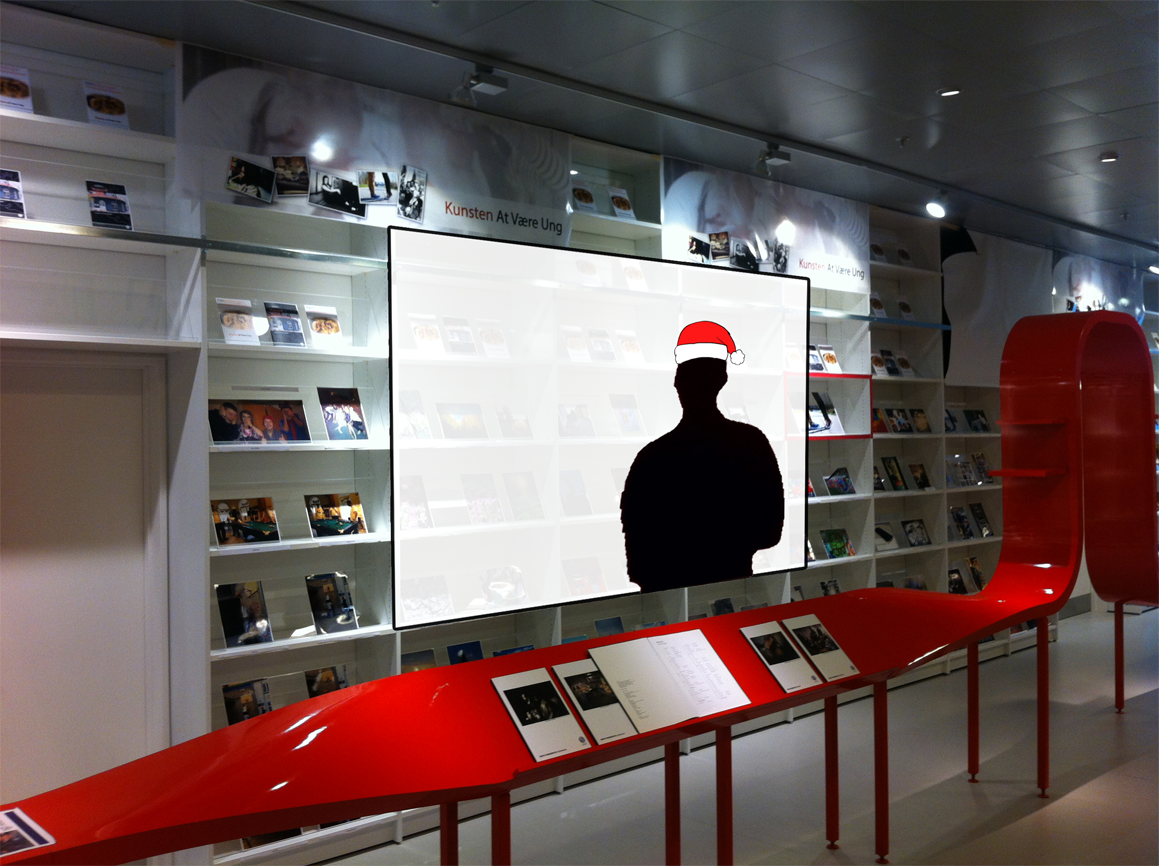
\includegraphics[width=1.00\textwidth]{Pictures/Hjørring Library/LocationJohannesHat.jpg}
\caption{Location at Hjørring Library}
\label{fig:Location at Hjørring Library}
\end{figure}



     


\section{This is awesome}
Yep yep

\begin{figure}[htbp]
\centering
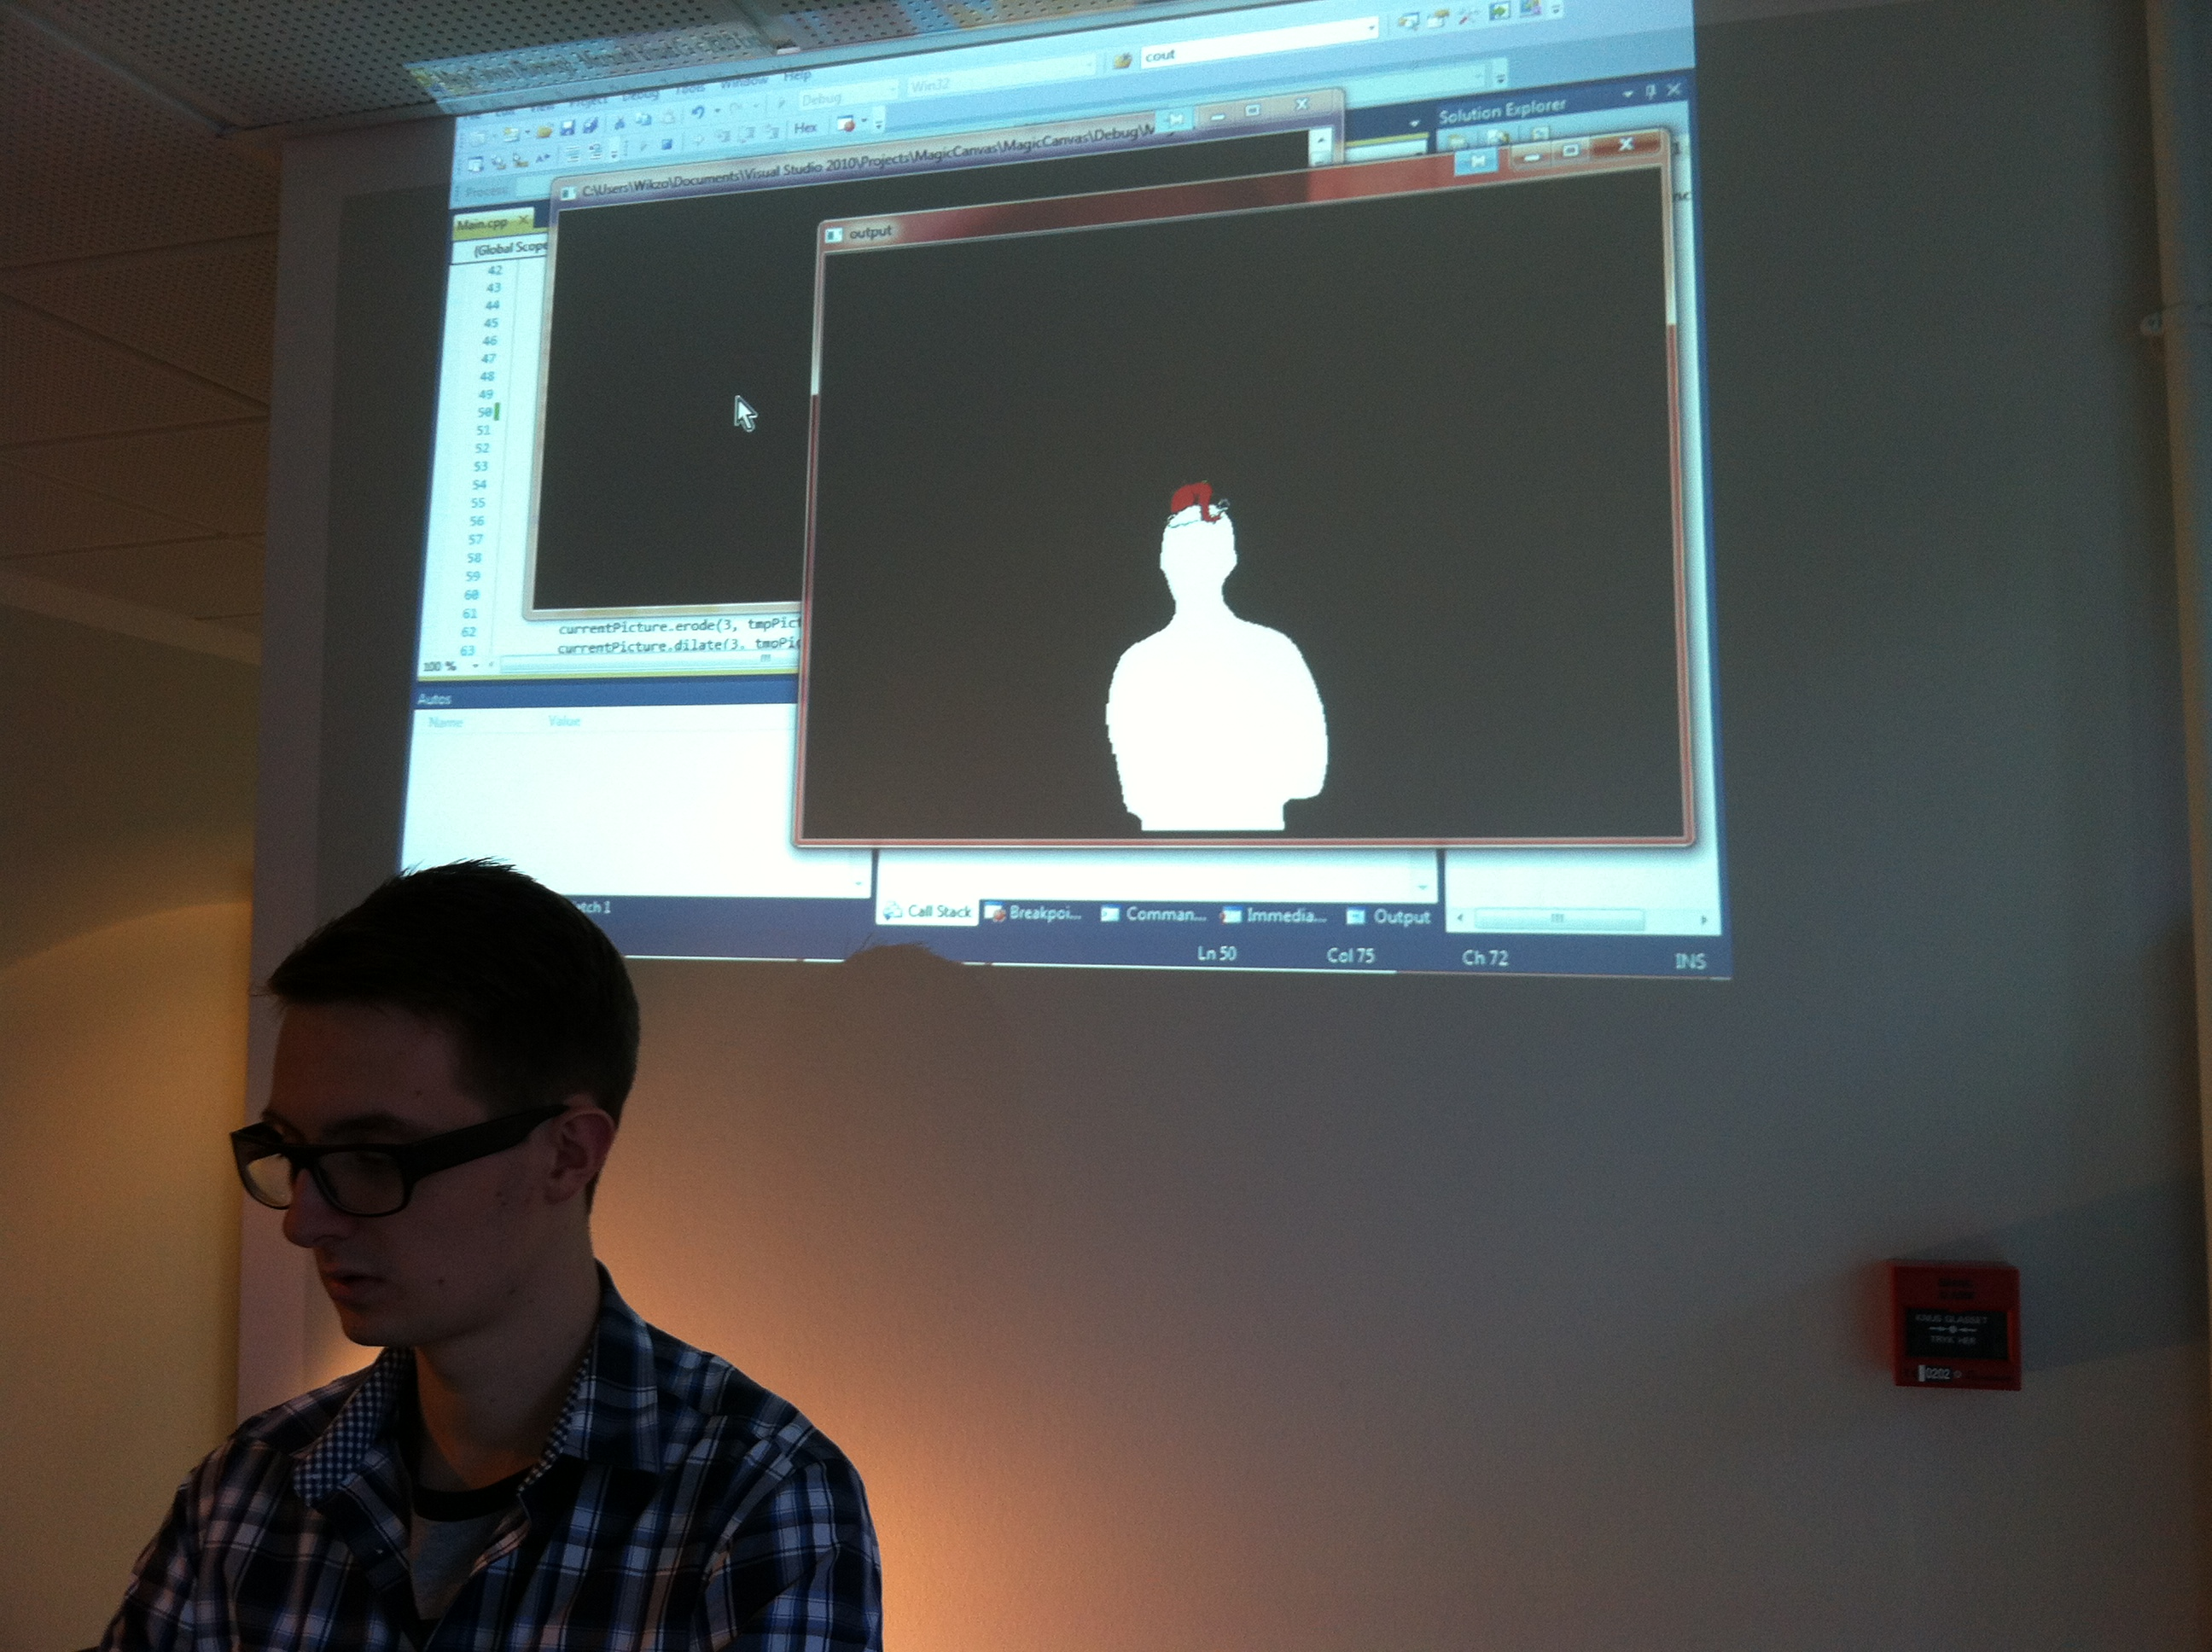
\includegraphics[width=1.00\textwidth]{Pictures/Test/IMG_1477.jpg}
\caption{Picture from Testing the Inferred Camera}
\label{fig:Picture from Testing the Inferred Camera}
\end{figure}

\subsection{Subway is good}
Nah...